% !TEX root = task-1-15-7.tex
% Editable task bank. Append new BankTask blocks at the end of the document.
\documentclass[12pt,a4paper]{article}
\usepackage{physics-textbook}
\usepackage{graphicx,needspace}
\usetikzlibrary{decorations.pathmorphing}
\newif\ifShowSolutions
\ifdefined\TutorEdition
  \ShowSolutionstrue
\else
  \ShowSolutionsfalse % Change to \ShowSolutionstrue to display solutions.
\fi
\newcounter{banktask}
\newsavebox{\BankTaskBox}
\newcommand{\BankTaskContent}[3]{%
  \noindent\textbf{\thebanktask.}\quad #2\par
  \ifShowSolutions
    \Needspace{50mm}% Keep the solution heading with its opening text or diagram.
    #3\par
    \ifdefined\TutorEdition
      \ifcsname TutorSource#1\endcsname
        \nopagebreak\smallskip{\small\csname TutorSource#1\endcsname\par}%
      \fi
    \fi
  \fi
}
\newcommand{\BankTask}[3]{%
  \refstepcounter{banktask}\par\medskip
  \sbox{\BankTaskBox}{\begin{minipage}{\linewidth}%
    \BankTaskContent{#1}{#2}{#3}\end{minipage}}%
  \ifdim\dimexpr\ht\BankTaskBox+\dp\BankTaskBox\relax>\dimexpr\textheight-20mm\relax
    \Needspace{35mm}\BankTaskContent{#1}{#2}{#3}%
  \else
    \Needspace{\dimexpr\ht\BankTaskBox+\dp\BankTaskBox\relax}%
    \noindent\usebox{\BankTaskBox}\par
  \fi
  \medskip
}
\begin{document}
\BookSubsection{1.15.7}{Закон сохранения механической энергии}


% Source sdamgia-410: https://phys-ege.sdamgia.ru/problem?id=410
\BankTask{sdamgia-410}{
Камень массой $1\,\text{кг}$ брошен вертикально вверх с начальной скоростью $4\,\text{м/с}$. На сколько увеличится потенциальная энергия камня от начала движения к тому времени, когда скорость камня уменьшится до $2\,\text{м/с}$?
}{
\smallskip\noindent\textbf{Решение}\par
Для камня выполняется закон сохранения полной механической энергии. Увеличение потенциальной энергии равно убыли кинетической энергии: 

\[\Delta E_{\text{пот}}= - \Delta E_{\text{кин}}= - ( \frac{m v _2 ^{2}}{2} - \frac{m v _1 ^{2}}{2} ) = - ( \frac{1 \cdot ( 2\,\text{м}/\text{с} ) ^{2}}{2} - \frac{1 \cdot ( 4\,\text{м}/\text{с} ) ^{2}}{2} ) =6\,\text{Дж}.\]

Ответ: $6$.
}

% Source sdamgia-505: https://phys-ege.sdamgia.ru/problem?id=505
\BankTask{sdamgia-505}{
Мальчик столкнул санки с вершины горки. Сразу после толчка санки имели скорость $5\,\text{м/с}$. Высота горки $10\,\text{м}$. Трение санок о снег пренебрежимо мало. Какова скорость санок у подножия горки? Ускорение свободного падения считать равным $10\,\text{м/с}^2$.
}{
\smallskip\noindent\textbf{Решение}\par
Поскольку трением санок о снег можно пренебречь, для них выполняется закон сохранения полной механической энергии. Пусть $m$ — масса санок, $h=10\,\text{м}$ — высота горки, $v =5\,\text{м}/\text{с}$ — начальная скорость, а $u$ — искомая скорость санок у подножия горки. Выпишем закон сохранения энергии (потенциальную энергию будем отсчитывать от низа горки):

\[\begin{gathered}\frac{m v ^{2}}{2} + mgh= \frac{mu ^{2}}{2} \Longleftrightarrow \frac{v ^{2}}{2} + gh= \frac{u ^{2}}{2},\end{gathered}\]
\[u= \sqrt{v ^{2} + 2gh} = \sqrt{5 ^{2} + 2 \cdot 10 \cdot 10} =15\,\text{м}/\text{с}.\]

Ответ: $15$.
}

% Source sdamgia-521: https://phys-ege.sdamgia.ru/problem?id=521
\BankTask{sdamgia-521}{
Брусок массой $m$ съезжает вниз по гладкой наклонной плоскости. Когда брусок опустится на высоту $h$ относительно первоначального положения, его полная механическая энергия\begin{enumerate}\item увеличится на величину $mgh$;\item уменьшится на величину $mgh$;\item не изменится;\item будет неизвестна, так как не задан угол наклона плоскости.\end{enumerate}
}{
\smallskip\noindent\textbf{Решение}\par
Поскольку брусок съезжает по гладкой наклонной плоскости, на него не действует сила трения, а значит, выполняется закон сохранения полной механической энергии. Когда брусок опустится на высоту $h$ относительно первоначального положения, его полная механическая энергия не изменится.

Ответ: $3$.
}

% Source sdamgia-744: https://phys-ege.sdamgia.ru/problem?id=744
\BankTask{sdamgia-744}{
Автомобиль, двигаясь с выключенным двигателем, на горизонтальном участке дороги имеет скорость $20\,\text{м/с}$. Какое расстояние он проедет до полной остановки вверх по склону горы под углом $30^\circ$ к горизонту? Трением пренебречь. Ускорение свободного падения считать равным $10\,\text{м/с}^2$.
}{
\smallskip\noindent\textbf{Решение}\par
Поскольку трением можно пренебречь, для автомобиля выполняется закон сохранения полной механической энергии. Кинетическая энергия поступательного движения автомобиля переходит в потенциальную. Высота, на которую автомобиль успевает подняться до полной остановки определяется из условия $\frac{m v ^{2}}{2} =mgh.$ Отсюда находим, что: 

\[h= \frac{v ^{2}}{2g} = \frac{( 20\,\text{м}/\text{с} ) ^{2}}{2 \cdot 10\,\text{м}/\text{с} ^{2}} =20\,\text{м}.\]

Следовательно, расстояние, которое автомобиль проедет вверх по склону горы до полной остановки, равно: 

\[S= \frac{h}{\sin 30 ^{\circ}} = \frac{20\,\text{м}}{1/2} =40\,\text{м}.\]

Ответ: $40$.
}

% Source sdamgia-4623: https://phys-ege.sdamgia.ru/problem?id=4623
\BankTask{sdamgia-4623}{
Тело, брошенное вертикально вверх с поверхности Земли, достигло максимальной высоты $5\,\text{м}$. С какой начальной скоростью тело было брошено вверх? Сопротивлением воздуха пренебречь. Ускорение свободного падения считать равным $10\,\text{м/с}^2$.
}{
\smallskip\noindent\textbf{Решение}\par
Поскольку сопротивлением воздух можно пренебречь, для тела выполняется закон сохранения энергии, а значит, вся начальная кинетическая энергия переходит в потенциальную энергию: $\frac{m v _0 ^{2}}{2} =mgh.$ Отсюда сразу находим начальную скорость: $v _0 = \sqrt{2gh} = \sqrt{2 \cdot 10\,\text{м}/\text{с} ^{2} \cdot 5\,\text{м}} = 10\,\text{м}/\text{с}.$

Ответ: $10$.
}

% Source sdamgia-7723: https://phys-ege.sdamgia.ru/problem?id=7723
\BankTask{sdamgia-7723}{
Мальчик бросил камень массой $100\,\text{г}$ под углом к горизонту из точки $A$. На рисунке в некотором масштабе изображена траектория $ABC$ полёта камня. \begin{center}\begin{tikzpicture}[task graph,x=.32cm,y=.32cm]
\draw[task grid,step=1] (0,0) grid (15,8);
\draw[task curve] (0,4)--(0,0)--(15,0);
\draw[task curve] (-3,4)--(0,4);
\foreach \x in {-3,-2.75,...,-.25}{\draw[task tick](\x,4)--++(-.18,-.18);}
\foreach \y in {.25,.5,...,3.75}{\draw[task tick](0,\y)--++(-.18,-.18);}
\foreach \x in {0,.25,...,15}{\draw[task tick](\x,0)--++(-.18,-.18);}
\draw[task curve,domain=0:12.549834,samples=80] plot (\x,{4+1.25*\x-.125*\x*\x});
\fill (0,4) circle(2pt) node[above left] {$A$};
\fill (8,6) circle(2pt) node[above right] {$B$};
\fill (12.549834,0) circle(2pt) node[above right] {$C$};
\draw[<->] (2,2)--(2,3) node[midway,right] {$1\,\text{м}$};
\end{tikzpicture}\end{center}Сопротивление воздуха пренебрежимо мало. В точке $B$ траектории модуль скорости камня был равен $8\,\text{м/с}$. Какую кинетическую энергию имел камень в точке $A$? Ускорение свободного падения принять равным $10\,\text{м/с}^2$.
}{
\smallskip\noindent\textbf{Решение}\par
Используем закон сохранения энергии. Потенциальную энергию будем отсчитывать от уровня точки $A$.

В таком случае, в точке $A$ камень обладает только кинетической энергией; в точке $B$ камень обладает и кинетической и потенциальной энергией.

Запишем закон сохранения энергии:

\[E_{\text{кин}A}=mgh_B + \frac{mV ^{2}}{2} =0{,}1 \cdot ( 10 \cdot 2 + \frac{8 ^{2}}{2} ) =5{,}2\,\text{Дж}.\]

Ответ: $5{,}2$.

Примечание:

Обратите внимание, что за нулевой уровень выбрана горизонталь, проходящая через точку $A$. Точка $B$ находится на высоте $2$ метров ($2$ клеточек) от этого уровня.
}

% Source sdamgia-50705: https://phys-ege.sdamgia.ru/problem?id=50705
\BankTask{sdamgia-50705}{
Шайбу массой $12\,\text{кг}$ толкают вверх по гладкой горке, она поднимается на максимальную высоту $h=4\,\text{м}$. Определите кинетическую энергию шайбы у основания горки. Сопротивлением воздуха пренебречь.
}{
\smallskip\noindent\textbf{Решение}\par
При отсутствии силы трения и сопротивления воздуха по закону сохранения энергии

\[E_{\text{к}1}=E_{\text{п}2}=mgh=12 \cdot 10 \cdot 4=480\,\text{Дж}.\]

Ответ: $480$.
}

% Source sdamgia-5629: https://phys-ege.sdamgia.ru/problem?id=5629
\BankTask{sdamgia-5629}{
На гладкой горизонтальной поверхности стола покоится горка с двумя вершинами, высоты которых $h$ и $\frac52h$ (см. рисунок). На правой вершине горки находится шайба. От незначительного толчка шайба и горка приходят в движение, причём шайба движется влево, не отрываясь от гладкой поверхности горки, а поступательно движущаяся горка не отрывается от стола. Скорость шайбы на левой вершине горки оказалась равной $v$. Найдите отношение масс шайбы и горки.\begin{center}\begin{tikzpicture}[book diagram,x=1cm,y=1cm]
\draw (0,0)--(5,0);\draw[book body,fill=gray!10] (0,0)..controls(.4,.8)and(.65,1.04)..(1.1,1.04)..controls(1.5,1.04)and(1.5,.4)..(1.9,.4)..controls(2.6,.4)and(2.6,2.6)..(3.7,2.6)..controls(4.5,2.6)and(4.6,1)..(4.8,0)--cycle;
\draw[book body] (3.55,2.6) rectangle (3.85,2.72);
\draw[<->] (-.25,0)--(-.25,1.04) node[midway,left] {$h$};
\draw[<->] (5,0)--(5,2.6) node[midway,right] {$\frac{5h}{2}$};
\end{tikzpicture}\end{center}
}{
\smallskip\noindent\textbf{Решение}\par
\begin{center}\begin{tikzpicture}[book diagram,x=.8cm,y=.8cm]
\foreach \yy/\xx/\label in {0/0/{t=0},-4/.5/{t=t_1}}{
\begin{scope}[shift={(0,\yy)}]
\draw[->] (0,0)--(5.3,0)node[right]{$x$};\draw[->](0,0)--(0,3.1)node[above]{$y$};\node[below left]at(0,0){$0$};
\begin{scope}[shift={(\xx,0)}]\draw[book body](0,0)..controls(.4,.8)and(.65,1.05)..(1.1,1.05)..controls(1.5,1.05)and(1.5,.4)..(1.9,.4)..controls(2.6,.4)and(2.6,2.7)..(3.6,2.7)..controls(4.2,2.7)and(4.4,1.5)..(4.7,0);\end{scope}
\node[above right]at(3.9,2.7){$\label$};
\end{scope}}
\draw[dashed](0,2.7)--(3.6,2.7);\node[left]at(0,2.7){$\frac{5h}{2}$};\draw[book body,fill=white](3.45,2.7)rectangle(3.75,2.85);
\draw[dashed](0,-2.95)--(1.6,-2.95);\node[left]at(0,-2.95){$h$};\draw[book body,fill=white](1.46,-2.95)rectangle(1.74,-2.81);
\draw[->](1.6,-2.6)--(.93,-2.6)node[midway,above]{$\vec v$};\draw[->](4.65,-2.7)--(5.3,-2.7)node[midway,above]{$\vec u$};
\end{tikzpicture}\end{center}

На систему тел «шайба — горка» действуют внешние силы (тяжести и реакции стола), но они обе направлены по вертикали, поэтому проекция импульса системы на горизонтальную ось $Ox$ системы отсчета, связанной со столом, сохраняется. 

В начальный момент $p_x=0,$ в конечный момент проекция полного импульса равна $p_x=Mu - m v .$ Из закона сохранения импульса получим: $Mu - m v =0,$ где $m$ — масса шайбы, $M$ — масса горки. 

Работа сил тяжести определяется изменением потенциальной энергии, а суммарная работа сил реакции равна нулю, так как поверхности гладкие. Следовательно, полная механическая энергия системы тел, равная сумме кинетической и потенциальной, сохраняется. Так как потенциальная энергия горки не изменилась, получаем уравнение 

\[\frac{m v ^{2}}{2} + \frac{Mu ^{2}}{2} + mgh= \frac{5}{2} mgh.\]

Решение системы дает отношение масс $\frac{m}{M} = \frac{3gh}{v ^{2}} - 1.$

Ответ: $\frac{m}{M} = \frac{3gh}{v ^{2}} - 1.$
}

% Source sdamgia-7642: https://phys-ege.sdamgia.ru/problem?id=7642
\BankTask{sdamgia-7642}{
К потолку на двух одинаковых лёгких пружинах общей жёсткостью $k=400\,\text{Н/м}$ подвешена чашка массой $m=500\,\text{г}$. С высоты $h=10\,\text{см}$ в чашку падает и прилипает к ней груз такой же массой $m$ (см. рисунок). На какое максимальное расстояние $H$ после этого опустится чашка относительно своего исходного положения? Потерями механической энергии пренебречь.\begin{center}\begin{tikzpicture}[book diagram]
\draw (0,2.7)--(3.2,2.7);
\draw (.4,2.7)--(.4,2.5);\draw plot[domain=0:1,samples=100]({.4+.08*sin(2880*\x)},{2.5-1.6*\x});\draw(.4,.9)--(.4,.7);
\draw (2.8,2.7)--(2.8,2.5);\draw plot[domain=0:1,samples=100]({2.8+.08*sin(2880*\x)},{2.5-1.6*\x});\draw(2.8,.9)--(2.8,.7);
\draw[book body] (.4,.7)..controls(1,-.1)and(2.2,-.1)..(2.8,.7);
\fill[gray] (1.6,2.2) circle(.12) node[above right,text=black] {$m$};
\node at(1.6,-.2){$m$};\node[left]at(.25,1.7){$k/2$};\node[right]at(2.95,1.7){$k/2$};
\draw[<->] (1.6,2.2)--(1.6,.1) node[midway,right] {$h$};\draw[->](4,2.4)--(4,1.8)node[right]{$\vec g$};
\end{tikzpicture}\end{center}
}{
\smallskip\noindent\textbf{Решение}\par
Груз, падая с высоты $h$ на чашку, в свободном падении приобретает скорость $V_1= \sqrt{2gh} .$ После абсолютно неупругого столкновения с чашкой той же массы, по закону сохранения импульса $mV_1=2mV_2$ находим начальную скорость чашки с прилипшим к ней грузом: $V_2= \frac{V_1}{2} = \sqrt{\frac{gh}{2}} .$

При дальнейшем движении чашки полная механическая энергия системы сохраняется. В нее в начальном состоянии входят кинетическая энергия чашки, потенциальная энергия чашки (относительно ее наинизшего положения), а также энергия упругой деформации пружин, а в конечном состоянии — только упругая энергия пружин:

\[\frac{2m \cdot V ^{2} _2}{2} + 2m \cdot gH + \frac{kh ^{2} _0}{2} = \frac{k ( h_0 + H ) ^{2}}{2} .\]

Начальное растяжение $h_{0}$ пружин находим из условия равновесия чашки до падения в нее груза: $mg=kh_0,$ откуда 

\[h_0= \frac{mg}{k} .\]

Подставляя в записанное выше соотношение выражения для скорости $V_{2}$ и величины $h_{0}$, получаем квадратное уравнение для определения искомой величины $H$:

\[kH ^{2} - 2mgH - mgh=0,\]

Откуда, с учетом положительности корня, для $H$ имеем:

\[H= \frac{mg}{k} ( 1 + \sqrt{1 + \frac{kh}{mg}} ) =5\,\text{см}.\]

Ответ: $5\,\text{см}$.
}

% Source sdamgia-4216: https://phys-ege.sdamgia.ru/problem?id=4216
\BankTask{sdamgia-4216}{
На тележке массой $M=400\,\text{г}$, которая может кататься без трения по горизонтальной плоскости, имеется лёгкий кронштейн, на котором подвешен на нити маленький шарик массой $m=100\,\text{г}$. На тележку по горизонтали налетает и абсолютно упруго сталкивается с ней шар массой $M$, летящий со скоростью $V_0=2\,\text{м/с}$ (см. рисунок). Чему будет равен модуль скорости тележки в тот момент, когда нить, на которой подвешен шарик, отклонится на максимальный угол от вертикали? Длительность столкновения шара с тележкой считать очень малой.\begin{center}\begin{tikzpicture}[book diagram]
\draw (-1,0)--(4,0);\draw[book body] (.5,.3)rectangle(3.5,.5);\draw (1,.15)circle(.15) (3,.15)circle(.15);
\draw (3.2,.5)--(3.2,2.6)--(2.2,2.6);\draw (2.2,2.6)--(2.2,1.2);\fill(2.2,1.2)circle(.12)node[right]{$m$};
\draw[book body](-.8,.5)circle(.17);\node[below]at(-.8,.35){$M$};\draw[->](-.5,.65)--(.3,.65)node[midway,above]{$V_0$};\node[above]at(1.3,.5){$M$};
\end{tikzpicture}\end{center}
}{
\smallskip\noindent\textbf{Решение}\par
Согласно условию, за время столкновения тележка практически не сместится, а нить останется вертикальной. В силу этого горизонтальная проекция силы натяжения нити во время столкновения отсутствует, и горизонтальная проекция импульса системы «шар + тележка» сохраняется: $MV_0=Mu_1 + Mu_2,$ где $u_1$ и $u_2$ — модули скоростей шара и тележки после столкновения. При абсолютно упругом столкновении шара и тележки сохраняется и их механическая энергия: $\frac{MV_0 ^{2}}{2} = \frac{Mu_1 ^{2}}{2} + \frac{Mu_2 ^{2}}{2} .$ Отсюда следует, что шар и тележка «обмениваются» скоростями: после столкновения шар останавливается и падает на плоскость, а тележка приобретает скорость $V_0.$

При дальнейшем движении тележка «уезжает» из-под подвешенного шарика, и нить начинает отклоняться от вертикали, постепенно тормозя тележку. В момент максимального отклонения нити от вертикали скорости $V$ тележки и шарика будут одинаковы, так как в противном случае, при скорости тележки большей, чем у шарика, отклонение нити будет продолжаться. В данном процессе сохраняется горизонтальная проекция импульса системы «шарик + тележка»:

$MV_0= ( M + m ) V.$ Отсюда $V= \frac{MV_0}{M + m} =1{,}6\,\text{м}/\text{с}.$

Ответ: $1{,}6\,\text{м/с}$.
}


% Source BD865C: https://ege.fipi.ru/bank/questions.php?search=1&proj=BA1F39653304A5B041B656915DC36B38&qid=BD865C
\BankTask{BD865C}{
Шайба соскальзывает по гладкой наклонной плоскости из состояния покоя
с высоты $80\,\text{см}$. Какова максимальная скорость шайбы у основания наклонной плоскости? Сопротивлением воздуха пренебречь. Результат выразите в $\text{м}/\text{с}$.
}{
\smallskip\noindent\textbf{Решение от GPT}\par
$mgh=mv^2/2$. При $h=0{,}8\,\text{м}$ получаем $v=\sqrt{2gh}=\sqrt{2\cdot10\cdot0{,}8}=4\,\text{м}/\text{с}$.
}

% Source B34015: https://ege.fipi.ru/bank/questions.php?search=1&proj=BA1F39653304A5B041B656915DC36B38&qid=B34015
\BankTask{B34015}{
Автомобиль с выключенным двигателем сняли со стояночного тормоза, и он покатился под уклон, составляющий угол $30\,{}^\circ$ с горизонтом. В начале горизонтального участка дороги, который следует за спуском, его скорость составляет $10\,\text{м}/\text{с}$. Какое расстояние автомобиль проезжает по склону? Трением пренебречь. Результат выразите в $\text{м}$.
}{
\smallskip\noindent\textbf{Решение от GPT}\par
$mgs\sin30^\circ=mv^2/2$. Тогда $s=v^2/(2g\sin30^\circ)=100/(2\cdot10\cdot0{,}5)=10\,\text{м}$.
}

% Source 12C0AE: https://ege.fipi.ru/bank/questions.php?search=1&proj=BA1F39653304A5B041B656915DC36B38&qid=12C0AE
\BankTask{12C0AE}{
Небольшой груз массой $0{,}1\,\text{кг}$ подвешен на невесомой нерастяжимой нити длиной $40\,\text{см}$. В результате толчка груз стал совершать незатухающие колебания в вертикальной плоскости. В таблице приведена зависимость от времени $t$ для высоты $h$ подъёма груза относительно положения равновесия.
\begin{center}{\small\setlength{\tabcolsep}{3pt}\begin{tabular}{|c|c|c|c|c|c|c|c|c|c|}\hline $t,\,\text{с}$ & $0$ & $0{,}2$ & $0{,}4$ & $0{,}6$ & $0{,}8$ & $1{,}0$ & $1{,}2$ & $1{,}4$ & $1{,}6$ \\\hline $h,\,\text{см}$ & $0$ & $12$ & $20$ & $12$ & $0$ & $12$ & $20$ & $12$ & $0$ \\\hline\end{tabular}}\end{center}
\begin{enumerate}
\item Период колебаний груза равен $0{,}8\,\text{с}$.
\item В момент времени $0{,}4\,\text{с}$ скорость груза максимальна.
\item В промежуток времени от $0{,}2$ до $1{,}0\,\text{с}$ кинетическая энергия груза достигла минимального значения $2$ раза.
\item В момент $1{,}2\,\text{с}$ кинетическая энергия груза равна $0$.
\item Максимальная скорость груза равна $2\,\text{м}/\text{с}$.
\end{enumerate}
}{
\smallskip\noindent\textbf{Решение от GPT}\par
При $t=1{,}2\,\text{с}$ груз на максимальной высоте, поэтому $E_{\text{к}}=0$. Из сохранения энергии $mv_{\max}^2/2=mgh_{\max}$: $v_{\max}=\sqrt{2\cdot10\cdot0{,}2}=2\,\text{м}/\text{с}$. Высота повторяется через полпериода, поэтому $T=1{,}6\,\text{с}$; на интервале $0{,}2\! -\!1{,}0\,\text{с}$ минимум кинетической энергии один. Ответ: $45$.
}

% Source ADDAE8: https://ege.fipi.ru/bank/questions.php?search=1&proj=BA1F39653304A5B041B656915DC36B38&qid=ADDAE8
\BankTask{ADDAE8}{
Тело брошено вертикально вверх с поверхности Земли в момент времени $t=0$. В таблице приведены результаты измерения модуля скорости тела в зависимости от времени.
\begin{center}{\small\setlength{\tabcolsep}{3pt}\begin{tabular}{|c|c|c|c|c|c|c|c|c|c|c|}\hline $t,\,\text{с}$ & $0{,}1$ & $0{,}2$ & $0{,}3$ & $0{,}4$ & $0{,}5$ & $0{,}6$ & $0{,}7$ & $0{,}8$ & $0{,}9$ & $1{,}0$ \\\hline $|v|,\,\text{м}/\text{с}$ & $4{,}0$ & $3{,}0$ & $2{,}0$ & $1{,}0$ & $0$ & $1{,}0$ & $2{,}0$ & $3{,}0$ & $4{,}0$ & $5{,}0$ \\\hline\end{tabular}}\end{center}
\begin{enumerate}
\item Тело поднялось на максимальную высоту, равную $0{,}8\,\text{м}$.
\item На высоте $0{,}8\,\text{м}$ от поверхности Земли скорость тела была равна $3{,}0\,\text{м}/\text{с}$.
\item Начальная скорость тела была равна $4\,\text{м}/\text{с}$.
\item В момент времени $t=0{,}9\,\text{с}$ тело находилось на высоте $0{,}45\,\text{м}$ от поверхности Земли.
\item В момент времени $t=0{,}2\,\text{с}$ тело находилось на высоте $0{,}45\,\text{м}$ от поверхности Земли.
\end{enumerate}
}{
\smallskip\noindent\textbf{Решение от GPT}\par
По таблице $g=10\,\text{м}/\text{с}^2$, $v_0=5\,\text{м}/\text{с}$. Высота $h=5t-5t^2$, $h_{\max}=1{,}25\,\text{м}$. На высоте $0{,}8\,\text{м}$ $v^2=v_0^2-2gh=9$, то есть $|v|=3\,\text{м}/\text{с}$. При $t=0{,}9\,\text{с}$ $h=4{,}5-4{,}05=0{,}45\,\text{м}$; при $0{,}2\,\text{с}$ $h=0{,}8\,\text{м}$. Ответ: $24$.
}

% Source F64C40: https://ege.fipi.ru/bank/questions.php?search=1&proj=BA1F39653304A5B041B656915DC36B38&qid=F64C40
\BankTask{F64C40}{
Искусственный спутник обращается вокруг Земли по вытянутой эллиптической орбите. В некоторый момент времени спутник проходит точку минимального удаления от Земли.
\begin{enumerate}
\item Кинетическая энергия спутника при прохождении этого положения максимальна.
\item Сила притяжения спутника к Земле в этом положении максимальна.
\item Полная механическая энергия спутника в этом положении достигает максимума.
\item Скорость спутника при прохождении этого положения минимальна.
\item Ускорение спутника при прохождении этого положения равно $0$.
\end{enumerate}
}{
\smallskip\noindent\textbf{Решение от GPT}\par
В перигее $r$ минимален, поэтому $F=GMm/r^2$ максимальна. Полная энергия постоянна; потенциальная $-GMm/r$ минимальна, следовательно, кинетическая энергия и скорость максимальны. Ответ: $12$.
}

% Source ACFD5A: https://ege.fipi.ru/bank/questions.php?search=1&proj=BA1F39653304A5B041B656915DC36B38&qid=ACFD5A
\BankTask{ACFD5A}{
Искусственный спутник обращается вокруг Земли по вытянутой эллиптической орбите. В некоторый момент времени спутник проходит положение максимального удаления от Земли.
\begin{enumerate}
\item Скорость спутника при прохождении этого положения максимальна.
\item Сила притяжения спутника к Земле при прохождении этого положения максимальна.
\item Полная механическая энергия спутника при прохождении этого положения максимальна.
\item Импульс спутника при прохождении этого положения минимален.
\item Ускорение спутника при прохождении этого положения минимально.
\end{enumerate}
}{
\smallskip\noindent\textbf{Решение от GPT}\par
В апогее $r$ максимален; поэтому $F=GMm/r^2$ и $a=GM/r^2$ минимальны. Полная механическая энергия постоянна, потенциальная максимальна, значит скорость и импульс минимальны. Ответ: $45$.
}

% Source F4CD91: https://ege.fipi.ru/bank/questions.php?search=1&proj=BA1F39653304A5B041B656915DC36B38&qid=F4CD91
\BankTask{F4CD91}{
Тело, брошенное с горизонтальной поверхности Земли со скоростью $v$ под углом $\alpha$ к горизонту, поднимается на максимальную высоту $h$ над земной поверхностью и затем падает на землю. Сопротивлением воздуха пренебречь.
\TaskMatchingColumns[.53\linewidth]{Физические величины}{
А) максимальная высота $h$ над горизонтом\par
Б) модуль вертикальной проекции скорости тела непосредственно перед падением на землю
}{Формулы}{
1) $\frac{v^2\sin^2\alpha}{2g}$\par
2) $v\sin\alpha$\par
3) $\frac{v^2\sin2\alpha}{2g}$\par
4) $v\cos\alpha$\par
}\begin{center}\begin{tabular}{|c|c|}\hline А & Б \\\hline\rule{0pt}{1.2em}\hspace{1cm} & \hspace{1cm} \\\hline\end{tabular}\end{center}
}{
\smallskip\noindent\textbf{Решение от GPT}\par
Начальная вертикальная скорость $v_{0y}=v\sin\alpha$. Из $v_y^2=v_{0y}^2-2gh$ при $v_y=0$ получаем $h=v^2\sin^2\alpha/(2g)$ (формула $1$). При возвращении на исходный уровень $v_y=-v\sin\alpha$, поэтому $|v_y|=v\sin\alpha$ (формула $2$). Ответ: $12$.
}

% Source DB3508: https://ege.fipi.ru/bank/questions.php?search=1&proj=BA1F39653304A5B041B656915DC36B38&qid=DB3508
\BankTask{DB3508}{
Шайба массой $m$ съезжает без трения из состояния покоя с вершины горки. У подножия горки потенциальная энергия шайбы равна нулю, а модуль её импульса равен $p$. Каковы высота горки и потенциальная энергия шайбы на её вершине? Ускорение свободного падения равно $g$.
\TaskMatchingColumns[.53\linewidth]{Физические величины}{
А) высота горки\par
Б) потенциальная энергия шайбы на вершине горки
}{Формулы}{
1) $\frac{p^2}{2m^2g}$\par
2) $\frac{p^2}{2mg}$\par
3) $\frac{p^2}{2m}$\par
4) $\frac{mp^2}{2g}$\par
}\begin{center}\begin{tabular}{|c|c|}\hline А & Б \\\hline\rule{0pt}{1.2em}\hspace{1cm} & \hspace{1cm} \\\hline\end{tabular}\end{center}
}{
\smallskip\noindent\textbf{Решение от GPT}\par
$mgh=mv^2/2=p^2/(2m)$. Поэтому $h=p^2/(2m^2g)$ (формула $1$), $E_{\text{п}}=p^2/(2m)$ (формула $3$). Ответ: $13$.
}

% Source 29461: https://phys-ege.sdamgia.ru/problem?id=29461
\BankTask{29461}{
\begin{center}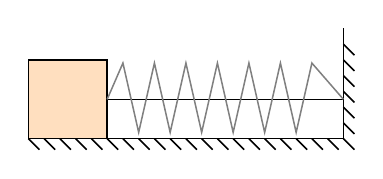
\begin{tikzpicture}[>=stealth,line width=.55pt]\draw[fill=orange!25](0,0)rectangle(1,1);\draw(0,0)--(4,0)--(4,1.4);\draw(1,.5)--(4,.5);\draw[gray](1,.5)--(1.2,.96)\foreach \x in {1.2,1.6,...,3.6}{--(\x+.2,.08)--(\x+.4,.96)}--(4,.5);\foreach \x in {0,.2,...,3.8}{\draw(\x,0)--++(.14,-.14);}\foreach \y in {0,.2,...,1.2}{\draw(4,\y)--++(.14,-.14);}\end{tikzpicture}\end{center}Нить, удерживающая легкую пружину в сжатом состоянии, внезапно оборвалась (см. рисунок). На сколько сантиметров была сжата пружина жесткостью $20\,\text{кН/м}$, если она сообщила бруску массой $20\,\text{г}$ максимальную скорость $10\,\text{м/с}$? Трением бруска о поверхность и массой пружины пренебречь.
}{
\smallskip\noindent\textbf{Решение}\par
В начальном положении в системе пружина обладала потенциальной энергией $E_p= \frac{kx ^2}{2} ,$ брусок находился в покое. Далее брусок приобретет максимальную скорость и кинетическую энергию $E_k= \frac{m v ^2}{2} ,$ когда пружина будет не деформирована. Учитывая, что работа сил тяжести и реакции опоры равна $0$, сила трения отсутствует, применяем закон сохранения энергии $E_p=E_k$ или $\frac{kx ^2}{2} = \frac{m v ^2}{2} .$ Откуда первоначальная деформация пружины: 

\[x= v \sqrt{\frac{m}{k}} =10 \cdot \sqrt{\frac{20\cdot10^{-3}}{20\cdot10^3}} =10 ^{ - 2 } \,\text{м}=1\,\text{см}.\]

Ответ: $1\,\text{см}$.
}

% Source 35160: https://phys-ege.sdamgia.ru/problem?id=35160
\BankTask{35160}{
Шар массой $1\,\text{кг}$, подвешенный на нити длиной $90\,\text{см}$, отводят от положения равновесия на угол $60$° и отпускают. В момент прохождения шаром положения равновесия в него попадает пуля массой $10\,\text{г}$, летящая навстречу шару. Она пробивает его и продолжает двигаться горизонтально. Определите модуль изменения импульса пули в результате попадания в шар, если он, продолжая движение в прежнем направлении, отклоняется на угол $39$°. (Массу шара считать неизменной, диаметр шара  — пренебрежимо малым по сравнению с длиной нити, $\cos 39 ^\circ = \frac{7}{9} .$) Какие законы Вы используете для решения задачи? Обоснуйте их применение.
}{
\smallskip\noindent\textbf{Решение}\par
Обоснование
$1$.  Введем инерциальную систему отсчета (ИСО), связанную с Землей.
$2$.  Тела движутся поступательно, размеры шарика малы по сравнению с размером нити, поэтому шарик и пулю можно описывать моделью материальной точки.
$3$.  Будем считать время взаимодействия пули и шарика малым, чтобы нить за время соударения не успела заметно отклониться. Тогда все силы в момент соударения направлены вертикально. Следовательно, в ИСО при попадании пули в шарик сохраняется горизонтальная составляющая импульса системы «шарик + пуля».
$4$.  После попадания пули в шарик при движении тел по вертикальной окружности механическая энергия равна сумме кинетической и потенциальной энергий тел $E=E_{\,\text{п}} + E_{\,\text{к}}.$ Изменение механической энергии тел в ИСО равно работе всех непотенциальных сил, приложенных к телу. Работа непотенциальной силы натяжения нити равна нулю, так как сила натяжения направлена перпендикулярно скорости в любой точке траектории.
$5$.  За нулевой уровень потенциальной энергии примем уровень положения равновесия шарика.

Перейдем к решению.
Потенциальная энергия равна $E_{\,\text{п}}=Mgh=Mgl ( 1 - \cos \alpha ) .$
Кинетическая энергия шарика в нижней точке $E_{\,\text{к}}= \frac{M v _0 ^2}{2} .$
По закону сохранения энергии:

\[Mgl ( 1 - \cos \alpha ) = \frac{M v _0 ^2}{2} .\]

Тогда скорость шарика в нижней точке равна:

\[v _0= \sqrt{2gl ( 1 - \cos \alpha )} .\]

Запишем законы сохранения импульса в момент удара и закон сохранения энергии после удара и до подъема шарика на максимальную высоту:

\[\begin{cases}Mv_0-mv_1=Mu-mv_2,\\ \dfrac{Mu^2}{2}=Mgl(1-\cos\beta).\end{cases}\]

Находим скорость шарика сразу после удара:

\[u= \sqrt{2gl ( 1 - \cos \beta )} .\]

Тогда изменение скорости пули равно:

$|\Delta v | = v _1 - v _2= \frac{M \sqrt{2gl}}{m} ( \sqrt{1 - \cos \alpha} - \sqrt{1 - \cos \beta} ) ;$
$|\Delta v|=\frac{1\cdot\sqrt{2\cdot10\cdot0{,}9}}{0{,}01}\left(\sqrt{1-0{,}5}-\sqrt{1-\frac79}\right)=100\,\text{м/с}.$

Модуль изменения импульса пули равен:

\[|\Delta p|=m|\Delta v |=0{,}01 \cdot 100=1 \,\text{кг} \cdot \,\text{м/с} .\]

Ответ: $1 \,\text{кг} \cdot \,\text{м/с} .$
}

% Source 25942: https://phys-ege.sdamgia.ru/problem?id=25942
\BankTask{25942}{
Небольшое тело массой $M$  =  $0{,}99\,\text{кг}$ лежит на вершине гладкой полусферы. В тело попадает пуля массой $m$  =  $0{,}01\,\text{кг}$, летящая горизонтально со скоростью $\upsilon_{0}$  =  $100\,\text{м/с}$, и застревает в нем. Пренебрегая смещением тела за время удара, определите радиус сферы, если высота, на которой тело оторвется от поверхности полусферы, $h$  =  $0{,}7\,\text{м}$. Высота отсчитывается от основания полусферы.
Какие законы Вы используете для описания взаимодействия тел? Обоснуйте их применение к данному случаю.
}{
\smallskip\noindent\textbf{Решение}\par
Обоснование 
Систему отсчета, связанную с Землей, будем считать инерциальной. Тела можно считать материальными точками, так как их размеры пренебрежимо малы в условии задачи. При соударении для системы «пуля  — тело» в ИСО выполняется закон сохранения импульса в проекции на горизонтальную ось, так как внешние силы (сила тяжести и сила реакции опоры) вертикальны.
При движении составного тела от вершины полусферы выполняется сохранение механической энергии, так как полусфера гладкая, и работа силы реакции опоры равна нулю (эта сила перпендикулярно скорости тела).
В момент отрыва обращается в ноль сила реакции опоры $\vec N.$
Второй закон Ньютона выполняется в ИСО для модели материальной точки.

Перейдем к решению.
$1$.  Запишем закон сохранения импульса в проекции на горизонтальную ось для столкновения пули и тела:

\[m v _0= ( M + m ) V_0.\]

Таким образом, тело с пулей начинают соскальзывать с начальной скоростью:

\[V_0= \frac{m v _0}{M + m} .\]

$2$.  Запишем закон сохранения энергии, чтобы найти скорость тела на высоте $h$ от Земли:

$\frac{( M + m ) V_0 ^2}{2} + ( M + m ) gR= \frac{( M + m ) V ^2}{2} + ( M + m ) gh,$
$V ^2 =V_0 ^2 + 2g ( R - h ) = ( \frac{m v _0}{M + m} ) ^2 + 2g ( R - h ) .$

$3$.  При движении тела по полусфере на него действуют сила тяжести и сила реакции опоры N.
В проекции на нормаль к поверхности полусферы второй закон Ньютона имеет вид:

\[( M + m ) a_{\,\text{ц}}= ( M + m ) \frac{V ^2}{R} = ( M + m ) g \cos \alpha - N.\]

Тело оторвется от поверхности в момент, когда сила реакции опоры будет равна нулю, при этом $\cos \alpha = \frac{h}{R} .$
Выражаем отсюда квадрат скорости тела:

\[V ^2 =gh.\]

$4$.  Подставим это значение в полученное ранее уравнение и найдем радиус полусферы:

$gh= ( \frac{m v _0}{M + m} ) ^2 + 2g ( R - h ) ,$
$R= \frac{3}{2} h - \frac{( m v _0 ) ^2}{2g ( M + m ) ^2} = \frac{3}{2} \cdot 0{,}7 - \frac{( 0{,}01 \cdot 100 ) ^2}{2 \cdot 10 \cdot ( 0{,}99 + 0{,}01 ) ^2} =1\,\text{м}.$

Ответ: $1\,\text{м}$.
}

% Source 19870: https://phys-ege.sdamgia.ru/problem?id=19870
\BankTask{19870}{
На двух невесомых нерастяжимых вертикальных нитях подвешена горизонтальная пробирка с газом, закрытая пробкой. Масса пробирки М  =  $0{,}05\,\text{кг}$, длина нитей $L$  =  $0{,}4\,\text{м}$, нить рвется, когда к ней прикладывается сила Т  =  $0{,}5$ Н. При нагревании подвешенной пробирки из нее вылетает пробка массой $m$ со скоростью $10\,\text{м/с}$. Найти минимальную массу пробки, при которой в момент ее вылета нити разорвутся.
}{
\smallskip\noindent\textbf{Решение}\par
$1$.  При взаимодействии пробки с пробиркой они приобретут скорости, равные соответственно $\upsilon$ и $u$. По закону сохранения импульса $m\upsilon=Mu$, откуда $m= \frac{Mu}{v} .$
$2$.  Пробирка приобретет скорость и в нижней точке по второму закону Ньютона $2$$T$ − Mg  =  Ma. При этом центростремительное ускорение пробирки равно $a= \frac{u ^2}{L} .$ Отсюда $u= \sqrt{\frac{L ( 2T - Mg )}{M}} .$
$3$.  Находим искомую массу пробки:

\[m= \frac{1}{v} \sqrt{ML ( 2T - Mg )} = \frac{1}{10} \sqrt{0{,}05 \cdot 0{,}4 \cdot ( 2 \cdot 0{,}5 - 0{,}05 \cdot 10 )} =0{,}01\,\text{кг} =10\,\text{г}.\]

Ответ: $10\,\text{г}$.
}

% Source 25758: https://phys-ege.sdamgia.ru/problem?id=25758
\BankTask{25758}{
Небольшая шайба после удара скользит вверх по наклонной плоскости из точки А (см. рис.).
\begin{center}\begin{tikzpicture}[task graph,>=stealth]\draw (0,0)--(5.8,0);\draw (0,0)--(4.5,1.38) arc (107:0:1.04);\draw (1,0) arc (0:17:1) node[midway,right]{\(\alpha\)};\begin{scope}[rotate=17]\draw[fill=gray!15] (0,0) rectangle(.85,.45);\draw[->](.85,.23)--(2,.23)node[above left]{\(\vec v_0\)};\end{scope}\node[below]at(0,0){\(A\)};\node[above]at(4.5,1.38){\(B\)};\draw[->](4.8,.39)--(5.55,1.12)node[midway,below right]{\(R\)};\end{tikzpicture}\end{center}
В точке В наклонная плоскость без излома переходит в наружную поверхность горизонтальной трубы радиусом R. Если в точке А скорость шайбы превосходит $v _0=4\,\text{м/с},$ то в точке В шайба отрывается от опоры. Длина наклонной плоскости $AB=L=1\,\text{м},$ угол $\alpha = 30 ^\circ.$ Коэффициент трения между наклонной плоскостью и шайбой $\mu =0{,}2.$ Найдите внешний радиус трубы R.
Какие законы Вы использовали для описания движения тела? Обоснуйте их применимость к данному случаю.
}{
\smallskip\noindent\textbf{Решение}\par
Обоснование 
$1$.  Рассмотрим задачу в системе отсчета, связанной с Землей. Будем считать эту систему отсчета инерциальной (ИСО). 
$2$.  Шайбу описываем моделью материальной точки, так как его размерами в данных условиях можно пренебречь.
$3$.  Поступательное движение шайбы происходит по шероховатой поверхности, поэтому на нее действует сила трения скольжения, равная $F_{\,\text{тр}}=\mu N.$
$4$.   На тело действуют потенциальная сила тяжести, сила реакции опоры и непотенциальная сила трения. Поскольку шайба описывается моделью материальной точки, то при движении тела по наклонной плоскости в ИСО работа силы трения равна изменению механической энергии.
$5$.  Для материальной точки условие отрыва шайбы от поверхности формулируется на основе второго закона Ньютона. В момент отрыва обращается в ноль сила реакции опоры. 
$6$.  В точке отрыва на тело действует только сила тяжести, которая является причиной ускорения свободного падения, направленного вертикально вниз и равная $10\,\text{м/с}^{2}$. Это же ускорение является центростремительным. Для модели материальной точки в ИСО применимы законы движения по окружности.

Перейдем к решению. 
По закону сохранения энергии в незамкнутой системе:

\[A_{\,\text{тр}}= E_{\,\text{пол}2} - E_{\,\text{пол}1},\]

где полная энергия в первом состоянии $E_{\,\text{пол}1}=E_{\,\text{к}1}= \frac{m v _0 ^2}{2} ,$ полная энергия во втором состоянии $E_{\,\text{пол}2}=E_{\,\text{к}2} + E_{\,\text{п}2}= \frac{m v _{\,\text{в}} ^2}{2} + mgh,$ причем высота подъема тела $h=L \sin \alpha .$ Работа силы трения $A_{\,\text{тр}}= - F_{\,\text{тр}}L,$ при этом сила трения скольжения $F_{\,\text{тр}}=\mu N.$ Из проекции на ось Oy $N=mg \cos \alpha .$
Объединяя формулы, получаем:

$\frac{m v _0 ^2}{2} =\mu mgL \cos \alpha + \frac{m v _B ^2}{2} + mgL \sin \alpha .$ ($1$)

В точке В условием отрыва будет равенство центростремительного ускорения $a= \frac{v _{\,\text{в}} ^2}{R}$ величине нормальной составляющей ускорения свободного падения:

$\frac{v _B ^2}{R} =g \cos \alpha ,$  откуда $v _B ^2 =Rg \cos \alpha .$($2$)

Из ($1$) и ($2$) находим внешний радиус трубы R:

\[R= \frac{v _0 ^2}{g \cos \alpha} - 2L ( \mu + \tan \alpha ) = \frac{16}{10 \cdot \cos 30 ^\circ} - 2 \cdot 1 \cdot ( 0{,}2 + \tan 30 ^\circ ) \approx 0{,}3\,\text{м}.\]

Ответ: R  =  $0{,}3\,\text{м}$.
}

% Source 25969: https://phys-ege.sdamgia.ru/problem?id=25969
\BankTask{25969}{
Пружинное ружье наклонено под углом $\alpha =30 ^\circ$ к горизонту. Энергия сжатой пружины равна $0{,}41\,\text{Дж}$. При выстреле шарик массой $m=50\,\text{г}$ проходит по стволу ружья расстояние b, вылетает и падает на расстоянии $L=1\,\text{м}$ от дула ружья в точку M, находящуюся с ним на одной высоте с дулом. (см. рис.). Найдите расстояние b. Трением в стволе и сопротивлением воздуха пренебречь.
Какие законы Вы использовали для описания движения шарика? Обоснуйте их применение к данному случаю.
\begin{center}\begin{tikzpicture}[task graph,>=stealth]\draw(0,0)--(4.6,0);\draw(0,0)--(4.6,2.75)--(10.2,2.75);\draw(0,0)--(-.25,.41)--(4.35,3.16)--(4.6,2.75);\draw[<->](1.2,1.2)--(4.31,3.06)node[midway,above]{\(b\)};\draw[<->](4.6,2.01)--(10.2,2.01)node[midway,below]{\(L\)};\draw(4.6,2.01)--(4.6,2.75)(10.2,2.01)--(10.2,2.75);\foreach \x in {4.7,4.85,...,10.1}{\draw(\x,2.75)--++(-.12,-.12);}\fill(10.2,2.75)circle(1.5pt)node[above right]{\(M\)};\draw(.72,0)arc(0:31:.72)node[midway,right]{\(\alpha\)};\begin{scope}[rotate=31]\draw plot[domain=.1:1.42,samples=120](\x,{.22+.13*sin(2727*\x)});\draw[fill=gray!15](1.63,.22)circle(.21)node[below right,xshift=2pt,yshift=-6pt]{\(m\)};\end{scope}\end{tikzpicture}\end{center}
}{
\smallskip\noindent\textbf{Решение}\par
Обоснование 
Систему отсчета, связанную с Землей, будем считать инерциальной. При движении пули по дулу пистолета на ее действуют силы тяжести, сила упругости и сила реакции опоры, не действуют сила трения (так как дуло можно считать абсолютно гладким) и сила сопротивления воздуха. В ИСО изменение полной механической энергии равно работе всех не потенциальных сил, действующих на тело. В данной задаче такой силой является сила реакции опоры $\vec N.$ Так как в процессе движения по стволу ружья сила реакции опоры $\vec N$ перпендикулярна поверхности, то ее работа равна нулю и $E_{\,\text{мех}}$ сохраняется в ИСО. 
При движении после вылета из трубки мы можем пренебречь действием силы сопротивления воздуха, значит, движение мяча происходит в поле Земного тяготения. Ось 0x направим горизонтально, ось 0y направим вертикально вверх. Тогда проекция вектора ускорения на ось 0x равна $0$, поэтому для описания движения по горизонтали можно использовать законы прямолинейного равномерного движения. Проекция вектора ускорения на ось 0y равна  — g, поэтому для описания движения по вертикали можно использовать законы прямолинейного равноускоренного движения.

Перейдем к решению.
$1$.  Рассмотрим движение шарика внутри трубки. По закону сохранения энергии $E_{\,\text{п}\,\text{пр}}=E_{\,\text{п}\,\text{ш}} + E_{\,\text{к}},$ где $E_{\,\text{п}\,\text{ш}}=mgh,$ $E_{\,\text{к}}= \frac{m v ^2}{2} .$ Откуда получаем:

\[E_{\,\text{пр}}=mgh + \frac{m v ^2}{2} .\]

По рисунку $h=b \cdot \sin \alpha .$
$2$.  Шарик вылетает из трубки со скоростью $v$ под углом $30 ^\circ$ к горизонту. При отсутствии сопротивления воздуха по горизонтальной оси движение равномерное, так как $g_x=0,$ по вертикальной оси, направленной вертикально вверх,  — равноускоренное с ускорением свободного падения, так как $g_y= - g.$ Такое движение описываем уравнениями $s_x= v _xt$ и $s_y= v _yt - \frac{gt ^2}{2} .$ Проекции начальной скорости при вылете из трубки $v _x= v \cos \alpha ,$ $v _y= v \sin \alpha .$ Учитывая, что в момент падения на горизонтальную плоскость $s_y=0,$ находим из приведенных формул время полета шарика: 

\[t= \frac{2 v \sin \alpha}{g} .\]

Тогда дальность полета шарика равна $L= \frac{v ^2 \sin 2 \alpha}{g} .$
$3$.  Объединяя записанные формулы, выразим искомую величину:

\[b= \frac{2E_{\,\text{пр}} \sin 2 \alpha - mgL}{2mg \sin \alpha \sin 2 \alpha} = \frac{2 \cdot 0{,}41 \cdot \sin 60 ^\circ - 0{,}05 \cdot 10 \cdot 1}{2 \cdot 0{,}05 \cdot 10 \cdot 0{,}5 \cdot \sin 60 ^\circ} \approx 0{,}485\,\text{м}=48{,}5\,\text{см}.\]

Ответ: $48{,}5\,\text{см}$.
}

% Source 29761: https://phys-ege.sdamgia.ru/problem?id=29761
\BankTask{29761}{
На горизонтальной поверхности неподвижно закреплена абсолютно гладкая полусфера радиусом $R=2{,}5$ м. С ее верхней точки из состояния покоя соскальзывает маленькое тело. В некоторой точке тело отрывается от сферы и летит свободно. Найдите скорость тела в момент отрыва от сферы. Сопротивлением воздуха пренебречь. Обоснуйте применимость используемых законов к решению задачи.
}{
\smallskip\noindent\textbf{Решение}\par
Обоснование
Систему отсчета, связанную с Землей, будем считать инерциальной. Поскольку размеры тела, соскальзывающего с полусферы, малы, то его можно считать материальной точкой. При движении тела от вершины полусферы выполняется закон сохранения механической энергии, так как полусфера гладкая, и работа силы реакции опоры равна нулю (эта сила перпендикулярна скорости тела). В момент отрыва обращается в ноль сила реакции опоры $\vec N .$ Второй закон Ньютона выполняется в ИСО для модели материальной точки.

Перейдем к решению.
$1$.  Рассмотрим два состояния системы  — в верхней точке полусферы и в точке отрыва от поверхности. В верхней точке шарик обладает потенциальной энергией $E_{p1}=m g h_1,$ причем $h_1=R.$ В точке отрыва от поверхности шарик обладает кинетической энергией $E_{k2}= \frac{m v ^2}{2}$ и потенциальной энергией $E_{p2}=m g h.$ Шарик при движении не вращается вследствие отсутствия силы трения, поэтому кинетической энергией вращения можно пренебречь.
По закону сохранения энергии:

\[m g R= \frac{m v ^2}{2} + m g h.\]

$2$.  Шарик отрывается от поверхности полусферы в том случае, когда сила реакции опоры становится равной нулю. На шарик действует сила тяжести, при движении по окружности ускорение направлено к центру окружности. Тогда по второму закону Ньютона в проекции на ось, совпадающую с вектором ускорения, получаем: $m a=m g \cos \alpha .$ Из рисунка видно, что $\cos \alpha = \frac{h}{R} .$ \begin{center}\begin{tikzpicture}[task graph,>=stealth]\draw(-2.04,0)--(3.08,0);\draw(1.6,0)arc(0:180:1.6);\draw(0,0)--(0,1.6)node[midway,left]{\(R\)};\filldraw[fill=gray!15](0,1.68)circle(.09) (1.13,1.13)circle(.09);\draw[dashed](0,0)--(1.13,1.13);\draw(1.13,1.13)--(3.08,1.13);\draw[<->](2.82,0)--(2.82,1.13)node[midway,right]{\(h\)};\draw(1.13,.8)arc(270:225:.33)node[midway,below left]{\(\alpha\)};\draw[->] (1.13,1.13)--(.49,.49) node[left]{\(\vec a\)};\draw[->] (1.13,1.13)--(1.13,-.55) node[right]{\(m\vec g\)};\end{tikzpicture}\end{center}
$3$.  При движении по окружности центростремительное ускорение равно $a= \frac{v ^2}{R} .$ 
$4$.  Объединяя формулы и решая совместно уравнения, выражаем скорость шарика в момент отрыва:

\[v = \sqrt{\frac{2 g R}{3}} = \sqrt{\frac{2 \cdot 10 \cdot 2{,}5}{3}} \approx 4{,}1 \,\text{м/с}.\]

Ответ: $4{,}1\,\text{м/с}$.
}

\end{document}
